\documentclass[oneside,a4paper,11pt]{book}
\usepackage[utf8]{inputenc}
\usepackage{svg}
\usepackage[italian]{babel}
\usepackage{float}
\usepackage{fancyvrb}
\usepackage{titling}
\usepackage[margin=1in,footskip=0.25in]{geometry}
\usepackage{listings}
\usepackage[DIV=12,BCOR=2mm,headinclude=true,footinclude=false]{typearea}
\usepackage{color, colortbl,xcolor}
\usepackage[hidelinks]{hyperref}
\usepackage{tcolorbox}
\usepackage{chngcntr}
\usepackage{calc}
\usepackage{amssymb}
\usepackage{subcaption}
\usepackage{amsthm}
\usepackage{amsfonts}
\usepackage{mathtools}
\usepackage{parskip}
\usepackage{cancel}
\usepackage{forest}
\usepackage{listings}
\usepackage{mathrsfs}
\usepackage{enumitem}
\usepackage{makecell}
%TIKZ environment
\usepackage{tikz}
\usepackage{pgfplots}
\pgfplotsset{compat=1.18}
\usepackage{fancyhdr}
\fancypagestyle{plain}{\fancyhf{}\renewcommand{\headrulewidth}{0pt}} % To clear page numbers from footer, and header line at the start of every chapter

\pagestyle{fancy}
\fancyhf{}% Clear header/footer
\fancyhead[L]{\nouppercase\leftmark}
\fancyhead[R]{\thepage}

\usetikzlibrary{positioning,shapes.geometric,arrows.meta,matrix,automata,decorations.pathmorphing,patterns,decorations.pathreplacing}
\tcbuselibrary{skins}
\counterwithin{figure}{section}
%Nuovi comandi
\newcommand\myeq{\stackrel{\mathclap{\normalfont\mbox{def}}}{=}}
\newcommand\prodG{\stackrel{\mathclap{\normalfont\mbox{\tiny{G}}}}{\Longrightarrow}}
%asmthm
\newlength{\marginlabelsep}\setlength{\marginlabelsep}{0.5em}
\newtheoremstyle{italicstyle} %% Name
  {} %% <- Space above (empty = default = \topsep = 8.0pt plus 2.0pt minus 4.0pt)
  {} %% <- Space below (empty = default = \topsep = 8.0pt plus 2.0pt minus 4.0pt)
  {\itshape} %% <- Body font
  {} %% <- Indent amount (empty = no indent, \parindent = just that)
  {\bfseries} %% <- Thm head font
  {} %% <- Punctuation after thm head
  {1pt} %% <- Space after thm head (or " " or \newline) (default: 5pt plus 1pt minus 1pt)
  {\vtop to 0pt{\llap{\thmname{#1}\hskip\marginlabelsep}
                \llap{\thmnumber{#2}\hskip\marginlabelsep}}\thmnote{#3\\}%
  }
\newtheoremstyle{normStyle} %% Name
  {} %% <- Space above (empty = default = \topsep = 8.0pt plus 2.0pt minus 4.0pt)
  {} %% <- Space below (empty = default = \topsep = 8.0pt plus 2.0pt minus 4.0pt)
  {\normalfont} %% <- Body font
  {} %% <- Indent amount (empty = no indent, \parindent = just that)
  {\bfseries} %% <- Thm head font
  {} %% <- Punctuation after thm head
  {1pt} %% <- Space after thm head (or " " or \newline) (default: 5pt plus 1pt minus 1pt)
  {\vtop to 0pt{\llap{\thmname{#1}\hskip\marginlabelsep}
                \llap{\thmnumber{#2}\hskip\marginlabelsep}}\thmnote{#3\\}%
  }
\theoremstyle{italicstyle}
\newtheorem{corollary}{Corollario}[section]
\newtheorem{notazione}{Notazione}[section]
\newtheorem{lemma}{Lemma}[section]
\newtheorem{definizione}{Definizione}[section]
\newtheorem{nota}{Nota}[section]
\newtheorem{exercise}{Esercizio}[section]


\theoremstyle{normStyle}
\newtheorem{exmp}{Esempio}[section]
\newtheorem{theorem}{Teorema}[section]
\newtheorem{proposizione}{Proposizione}[section]

\tcbuselibrary{listings,skins}
\newtcblisting{mylisting}[2][]{
        arc=0pt, outer arc=0pt,
    listing only, 
    title=#2,
    #1,
    listing options= {escapechar=|}
}

\newcommand{\myboxedtext}[2][rectangle,draw]{%
        \tikz[baseline=-0.6ex] \node [#1]{#2};}%
\title{Programmazione e Sicurezza delle Reti}
\author{Alessio Gjergji}
\date{Anno accademico 2022 - 2023}

\begin{document}
\hypersetup{ %set true if you want colored links
    linktoc=all,     %set to all if you want both sections and subsections linked
    linkcolor=black,  %choose some color if you want links to stand out
}
\maketitle
\tableofcontents
\chapter{Ripasso di Reti di Calcolatori}
\section{Concetti di base}
Lo stack \textbf{TCP/IP} è composto da vari livelli:
\begin{itemize}
  \item Applicazione
  \item Trasporto 
  \item Rete
  \item Collegamento dati 
  \item Fisico
\end{itemize}
\section{Livello di Applicazione}
\subsection{Architetture delle applicazioni di rete}
Le architetture delle applicazioni di rete possono essere:
\begin{itemize}
  \item Client - Server.
  \item Peer-to-Peer.
  \item Architetture ibride.
\end{itemize}
\subsubsection{Architettura client-server}
Il server è un host sempre attivo, composto da indirizzo IP fisso, mentre 
il client comunica con il server in qualunque momento esso voglia. Il client 
può avere IP dinamici e non comunica direttamente con altri client.
\subsubsection{Architettura P2P}
Tale architettura è caratterizzata da un server non sempre attivo, infatti 
coppie arbitrarie di host, detti peer, comunicano direttamente tra loro. I peer 
non devono necessariamente essere sempre attivi, e cambiano indirizzo IP.
\subsection{Servizi di trasporto di un'applicazione}
\begin{itemize}
  \item Affidabilità: alcune applicazioni possono tollerare qualche perdita 
  di pacchetto, mentre altre non le tollerano.
  \item Ritardi: alcune applicazioni per essere "realistiche" richiedono bassi 
  ritardi o bassa variazione del ritardo.
  \item Throughput: alcune applicazioni per essere "efficaci" richiedono almeno una certa 
  capacità del canale.
  \item Sicurezza: cifratura, integrità dei dati, autenticazione.
\end{itemize}
\section{Livello di Trasporto}
\subsection{Socket}
Il socket è una tupla che identifica il flusso tra due
applicazioni su host anche molto distanti tra loro. Esso 
è composto da \textbf{Sourece address}, \textbf{Destination Address},
\textbf{Source Port}, \textbf{Destination Port}.

Per Host intendiamo un sistema di elaborazione che ospita
applicazioni di rete. Possono essere terminali, e tutti i
dispositivi che si collegano in rete. Esse ospitano le
applicazioni che utilizzano gli utenti.

L'applicazione di rete è l'interazione di diversi processi, i processi
sono programmi (\textit{sequenza di istruzioni}) in esecuzione.
Avere due host su internet fa si che essi debbano avere un indirizzo IP che li
identifichi e per comunicare si scambiano pacchetti per comunicare. Ai due host potrebbere
corrispondere più host e perciò a livello di trasporto viene istituito anche 
un ulteriore valore chiamato porta.

\subsection{User Datagram Protocol}
Si tratta di un protocollo di trasporto connectionless non affidabile. Esso
svolge solo la funzione di indirizzamento delle applicazioni (\textit{porte}).

Permette di costruire applicazioni con sole due primitive \textbf{send} e 
\textbf{recive}.
A livello IP non sono sicuro che il pacchetto arrivi effetivamente a 
destinazione, è infatti utilizzato per il supporto di transazioni semplici tra applicativi
e per applicazioni multimendiali.
\subsection{Transport Control Protocol}
I pacchetti TCP contiene un header più ricco perchè si tratta di un protocollo
orientato alla connessione dove la perdita di pacchetti implica il rinvio dei pacchetti persi.
Il protocollo TCP fornisce affidabilità e consegna ordinata.
L'header include:
\begin{itemize}
  \item Source port - Destination port (\textit{16 bit}): indirizzi della porta
  sorgente e della porta destinazione.
  \item Sequence number (\textit{32 bit}): numero di sequenza del primo byte del payload.
  \item Acknowledge Number (\textit{32 bit}): numero di sequenza del prossimo byte che si intende 
  ricevere (ha la validità di un segmento ACK).
  \item Offest (\textit{4 bit}): lunghezza dell'header TCP, in multipli di 32 bit.
  \item Reserved (\textit{6 bit}): riservato per usi futuri
  \item Window (\textit{16 bit}) ampiezza della finestra di ricezione (comunicato
  dalla destinazione alla sorgente).
  \item Checksum (\textit{16 bit}): risultato di un calcolo che serve per sapere se
  il segmento corrente contiene errori nel campo dati.
  \item Urgent Pointer (\textit{16 bit}): indica che il ricevente deve iniziare a 
  leggere il campo dati a partire dal numero di byte specificato.
  Viene usato se si inviano 
  comandi che danno inizio ad eventi asincroni "urgenti".
  \item Flag (\textit{1 bit}):
  \begin{itemize}
    \item URG: vale uno se vi sono dati urgenti; 
    in questo caso il campo urgent pointer ha senso.
    \item ACK: vale uno se il segmento è un ACK valido; 
    in questo caso l’acknowledge number contiene un numero valido.
    \item PSH: vale uno quando il trasmettitore intende usare il comando di PUSH.
    \item RST: reset; resetta la connessione senza un tear down esplicito.
    \item SYN: synchronize; usato durante il setup per comunicare i numeri di sequenza iniziale.
    \item FIN: usato per la chiusura esplicita di una connessione.
  \end{itemize}
  \item Option and Padding (\textit{lunghezza variabile}):  riempimento (fino a multipli di 32 bit) e campi 
  opzionali come ad esempio durante il setup per comunicare il MSS.
  \item Data: i dati provenienti dall’applicazione.
\end{itemize}
Con il TCP avremo quindi 4 chiamate a funzione.
\begin{itemize}
  \item Apertura della connessione.
  \item Send.
  \item Recive.
  \item Chiusura della connessione.
\end{itemize}
\subsubsection{Instaurazione della connessione}
Il TCP è un protocollo \textbf{connection oriented}, ciò significa 
che prima di iniziare a trasferire i dati ci si deve essere 
una connessione tra due end-system.

L'instaturazione della connessione avviene secondo la procedura 
"three-way handshake"
\begin{itemize}
  \item la stazione che richiede la connessione (A) invia un segmento SYN.
  \item la stazione che riceve la richiesta (B) risponde con un segmento
  SYN.
  \item la stazione A riscontra il segmento SYN della stazione B.
\end{itemize}
\subsubsection{Terminazione della connessione}
Poiché la connessione è bidirezionale, la terminazione deve avvenire in entrambe le direzioni.
\begin{itemize}
  \item la stazione che non ha più dati da trasmettere e decide
  di chiudere la connessione invia un segmento FIN (semgneto con il campo FIN a 1 e il campo dati vuoto).
  \item la stazione che riceve il segmento FIN invia un ACK e indica all'applicazione che la comunicazione 
  è stata chiusa nella direzione entrante.
  \item Per chiudere completamente la connessione, la procedura 
  di half close deve avvenire anche nell'altra direzione.
\end{itemize}
\subsubsection{Stima del Round Trip Time}
Poichè l'RTT può variare anche molto in base alle condizioni della rete, 
il valore di RTT (SRTT Smoothed RTT) utilizzato per il calcolo di RTO risulta una stima del valor medio 
di RTT sperimentato dai diversi segmenti.
\[
  SRTT_{attuale} = (\alpha \cdot SRTT_{precedente})+((1-\alpha)\cdot RTT_{istantaneo})
\]
Dove:
\begin{itemize}
  \item $RTT_{istantaneo}$: misura di RTT sull'ultimo segmento.
  \item $RTT_{precedente}$: stima precedente del valore medio di RTT.
  \item $SRTT_{attuale}$: stima attuale del valore medio di RTT.
  \item $\alpha$: coefficientedi peso compreso tra zero e uno.
\end{itemize}
\subsubsection{Stima del Retrasmition Time Out}
\[
  RTO = \beta \cdot SRTT
\]
La sorgente, dunque, attende fino a due volte il RTT medio (SRTT) 
prima di considerare il segmento perso e ritrasmetterlo.

In caso di ritrasmissione, il RTO per quel segmento viene ricalcolato
in base ad un processo di exponential backoff.
\subsection{Interazione tra Router e Forwarding}
La rete internet è tenuta insieme dai router, i router fanno
due operazioni, il routing e il forwarding.

Il routing è il processo di scoperta del cammino da una sorgente ad ogni destinazione
nella rete. Un protocollo di routing gestisce una tabella di routing nei router, la tabella
indica, per ongi destinazione, qual è l'interfaccia di uscita su cui inviare il pacchetto.
Gli algoritmi utilizzati per risolvere tale problema sono:
\begin{itemize}
  \item Distance Vector: periodicamente ogni nodo invia ai propri vicini il
  vettore delle distanze verso tutte le sottoreti del mondo.
  \item Link State: periodicamente ogni nodo invia a tutte le sottoreti 
  del mondo lo stato dei collegamenti verso i propri vicini.
\end{itemize}

Il forwarding consiste nel scegliere l'interfaccia
di uscita adatta sulla quale incanalare il pacchetto. 
\section{Livello di Rete}
\subsection{Gerarichia degli indirizzi IP}
Gli indirizzi IP sono divisi in due parti:
\begin{itemize}
  \item Un prefisso: identifica la rete fisica a cui l'host è connesso, 
  anche noto come \textbf{NetID}. A ciascuna rete in Internet viene assegnato 
  un prefisso di rete univoco.
  \item Un suffisso: identifica un host specifico all'interno  di una 
  rete, anche noto come \textbf{HostID}. A ciascun host su una data rete viene 
  assegnato un suffisso univoco mentre il prefisso è uguale per tutti.
\end{itemize}
Lo schema degli indirizzi IP garantisce due proprietà:
\begin{itemize}
  \item A ciascun host viene assegnato un indirizzo unico.
  \item L'assegnazione dei numeri di rete (prefissi) viene coordinata 
  globalmente, mentre i prefissi vengono assegnati localmente.
\end{itemize}
\subsubsection{Subnet e indirizzamento classes}
I prefissi sono di lunghezza fissa ed hanno indirizzamento classful (\textit{4 classi}).
Tale schema, con l'espansione di internet si è rilevato limitante, siccome tutti richiedevano 
l'utilizzo di indirizzi di classe A e B in modo da poter avere un numero sufficiente di indirizzi 
per eventuali espansioni. La conseguenza fu il sottoutilizzo di indirizzi all'interno di ogni classe.
\subsection{Notazione Classless-Domain Routing}
L'utilizzo di maschere per specificare la dimensione del prefisso viene fatta per 
questioni di efficienza, poichè le operazioni di AND bit a bit sono molto veloci in hardware.

Tuttavia, per facilitare la gestione da parte degli utenti, si utilizza una
notazione più semplice e diretta, specificando la dimensione del prefisso.
\[
  ddd.ddd.ddd.ddd/m
\]
dove:
\begin{itemize}
  \item $ddd$ è il valore decimale nella notazione puntata.
  \item $m$ è il numero di bit del prefisso.
\end{itemize}
\paragraph*{Esempio}
\begin{itemize}
  \item NetA: $128.10.0.0/16$
  \item NetB: $64.10.2.0/24$
\end{itemize}
\subsection{Interfacce di rete}
Gli indirizzi non sono dati alle macchine, ma alle interfacce, quindi su 
un dispositivo possono essere molteplici. 
\section{Livello di Collegamento Dati}
Le principali funzioni svolte dal livello 2 sono:
\begin{itemize}
  \item Framing: delimitazione dei messaggi (\textit{frame}) come gruppi 
  di bit sul canale fisico.
  \item Rilevazione/gestione errori: controlla se il frame contiene errori ed 
  eventualemente gestisce il recupero.
  \item Metodo di accesso al canale.
  \item Controllo di flusso: gestisce la velocità della trasmissione.
\end{itemize}
\subsection{Framing}
Il livello 2 riceve dal livello superiore (\textit{rete}) dei pacchetti.
Considerando che:
\begin{itemize}
  \item La lunghezza dei pacchetti (\textit{di livello 3}) e delle corrispondenti 
  trame (\textit{livello 2}) è variabile.
  \item I sistemi non sono sincronizzati tra loro.
  \item Il livello 1 tratta solo bit, e quindi non è in grado di distinguere se un bit appartiene 
  \item ad una trama o a quella successiva.
\end{itemize}
Nasce quindi il problema della \textbf{delimitazione dei frame}. La 
funzionalità di framing è dunque rendere distinguibile un frame dall'altro attraverso 
l'utilizzo di opportuni codici all'inizio e alla fine del frame stesso.
\subsection{Metodo di accesso al canale}
La modalità di trasmissione di distingue in:
\begin{itemize}
  \item Punto - punto: dove la trasmissione è limitata ai dispositivi.
  \item Broadcast: dove la limitazione non è più presente.
\end{itemize}
La metodologia Broadcast richiede l'implementazione di tecniche di allocazione:
\begin{itemize}
  \item Statica: TDM, FDM, CDM, \dots 
  \item Dinamica.
\end{itemize}
L'allocazione dinamica richiede la suddivisione in due categorie nella 
tecnica di assegnazione:
\begin{itemize}
  \item A turno: token ring, token pass, \dots
  \item A contesa: Aloha, Slotted Aloha, CSMA, CSMA-CD, \dots
\end{itemize}

\chapter{Dal Web ai Webservices}
\section{HTTP/HTTPS}
I protocolli HTTP e HTTPS è nato per la fruizione dei contenuti in rete (\textit{World Wide Web}). 
Oggi è utilizzato anche per l'invocazione di funzionalità remote, i \textbf{webservice}.

Il client si chiama "web browser" (\textit{o semplicemente "browser"}) e la 
comunicazione avviene sul protocollo TCP sulla rete internet.

L'apertura della comunicazione avviene attraverso gli attori \textit{client} e 
\textit{server} identificati rispettivamente da indirizzo ip e porta (\textit{l'HTTP 
utilizza la porta $80$, l'HTTPS utilizza la porta $443$}). 
L'HTTP viaggia sul protocollo TCP e la prima cosa da eseguire è l'apertura della
connessione (\textit{attraverso il tree way handshake}). 
Una volta effettuata l'apertura della connessione si identifica da soli richieste seguite da 
risposte.
Nel caso di HTTPS avviene l'autenticazione del server e la negoziazione 
di una chiave di cifratura.

Si tratta di un protocollo testuale, leggibili.

\subsubsection{Esempio}
\begin{lstlisting}[basicstyle=\small]
GET /it/i-nostri-servizi/servizi-per-studenti HTTP/1.1
User-Agent: Mozilla/5.0 (X11; U; Linux i686; en-US; rv:1.9.1.8)
Gecko/20100214 Ubuntu/9.10 (karmic) Firefox/3.5.8
Accept: text/html,application/xhtml+xml,application/xml;q=0.9,*/*;q=0.8
Accept-Language: en-us,en;q=0.5
Accept-Encoding: gzip,deflate
Accept-Charset: ISO-8859-1,utf-8;q=0.7,*;q=0.7
Keep-Alive: 300
Connection: keep-alive
\end{lstlisting}
\subsection{Esempio di risposta}
\begin{lstlisting}[basicstyle=\small]
HTTP/1.1 200 OK
Date: Mon, 17 May 2022 16:10:48 GMT
Server: Apache
Last-Modified: Mon, 29 Mar 2022 13:57:17 GMT
Keep-Alive: timeout=15, max=100
Connection: Keep-Alive
Transfer-Encoding: chunked
Content-Type: text/html

<html> 
  ... 
</html>
\end{lstlisting}
\section{Metodi di richiesta HTTP}
\begin{itemize}
  \item GET: imposta i parametri nella URL, con il limite di $2048$ caratteri.
  \item POST: imposta i dati nel corpo della richiesta, dove non c'è limite di 
  caratteri.
  \item PUT 
  \item DELETE 
  \item HEAD 
  \item CONNECTION 
  \item OPTIONS 
  \item TRACE 
  \item PATCH 
\end{itemize}
\section{HTTPS}
I messaggi che passano nella connessione TCP sono gli stessi dell'HTTP ma vengono 
sottoposti a cifratura dei dati in transito e autenticazione del server mediante 
certificato digitale.

Il server lavora sulla porta $443$ invece che $80$.
\section{Service-oriented architecture}
Le tradizionali applicazioni "monolitiche" sono costituite da l'interfaccia utente che 
richiama delle funzionalità fornite da una serie di \textbf{librerie} linkate 
in un unico programma che "gira" sulla macchina dell'utente.

Le SOA hanno l'obiettivo di realizzare applicazioni complesse attraverso la 
\textbf{combinazione di diversi programmi attraverso la rete}.
\begin{itemize}
  \item L'interfaccia utente più qualche funzionalità di base "girano" sull'host dell'utente.
  \item Le funzionalità principali dell’applicazione sono fornite da programmi che girano su uno o più server.
\end{itemize}
\subsection{Vantaggi}
\begin{itemize}
  \item Potenza di calcolo e memoria sono delegate ai server;
  \item Protezione della proprietà intellettuale su algoritmi strategici;
  \item Annullamento della necessità di distribuire aggiornamenti del software ;
  quando le modifiche riguardano solo il codice dei server;
  \item Nuovo modello economico: pay per use;
  \item Eliminazione della pirateria;
  \item L’infrastruttura di rete diventa un elemento essenziale;
  \item Se “manca la rete” l’applicazione non funziona.
\end{itemize}
\section{Applicazioni client server}
I client e i server possono essere molteplici, questo protocollo 
è contraddistinto dal client che esegue il primo passo.
Client e server sono processi e non host, l'insieme 
di almeno un client e un server costituisce l'applicazione 
di rete.

Per testare non serve necessariamente una connessione alla rete ma si 
può usare una rete fittizia chiamata loopback. In tal caso l'interfaccia 
socket sia del client sia del server hanno indirizzo IP $127.0.0.1$ chiamata
\textbf{localhost}.

Le interfacce create da parte del client e del server devono essere 
create su porte diverse e il client deve conoscere la porta del server.
\subsection{Protocollo UDP}
Il sistema operativo mette a disposizione un'API per agire sulla 
rete, utilizzando i protocolli a livello di trasporto.
\subsubsection{Client}
Il client esegue delle richieste al server attraverso 
queste modalità:
\begin{itemize}
  \item Inizio;
  \item Dichiarazione delle variabili tra cui la variabile socket;
  \item Inizializzazione dell’interfaccia socket sulla porta $20000$;
  \item Invia tramite UDP il messaggio "Ciao sono il client!" al destinatario avente indirizzo IP "127.0.0.1" e porta 35000;
  \item Mettiti in attesa dell’arrivo di un messaggio UDP;
  \item Scrivi "\verb|[CLIENT]| Ho ricevuto un messaggio da";
  \item Scrivi host/porta del mittente e contenuto ricevuto.
  \item Fine.
\end{itemize}

\subsubsection{Server}
Il server attende delle richieste da parte del client seguendo 
questi passaggi:
\begin{itemize}
  \item Inizio;
  \item Dichiarazione delle variabili tra cui la variabile socket;
  \item Inizializzazione dell’interfaccia socket sulla porta $35000$;
  \item Scrivi "\verb|[SERVER]| Sono in attesa di richieste da qualche client";
  \item Mettiti in attesa dell’arrivo di un messaggio UDP;
  \item Scrivi "\verb|[SERVER]| Ho ricevuto un messaggio da";
  \item Scrivi host/porta del mittente e contenuto ricevuto;
  \item Invia a tale mittente tramite UDP il messaggio "Sono il server: ho ricevuto correttamente il tuo messaggio!";
  \item Fine.
\end{itemize}
\subsection{Come scrivere applicazioni di rete}
\subsubsection{Creazione dell'interfaccia socket}
Tutti i sistemi operativi forniscono un'interfaccia software per 
costruire questi programmi con un qualsiasi linguaggio di programmazione.
Questa interfaccia si chiama \textbf{socket}.

Il programma prima di usare la rete deve creare un oggetto di tipo socket definito 
da tre parametri:
\begin{itemize}
  \item Indirizzo IP locale;
  \item Porta locale (\textit{si aggancia al processo in esecuzione});
  \item Modalità di trasmissione: UDP oppure TCP.
\end{itemize}

Il server deve decidere esplicitamente il numero di porta locale affinché i 
client possano saperlo. Gli indirizzi compresi tra $0$ e $1023$ sono riservati 
a protocolli applicativi noti, in questo caso il programma che crea un oggetto 
socket su queste porte deve avere i privilegi di root.

Il programma \textbf{client} può deciderlo esplicitamente oppure lasciarlo decidere 
al proprio sistema operativo.
\subsubsection{La trasmissione/ricezione}
Per tale fase serve conoscere ulteriori parametri:
\begin{itemize}
  \item IP del proprio interlocutore;
  \item Porta del proprio interlocutore.
\end{itemize}
Nel caso UDP:
\begin{itemize}
  \item Chiamata a funzione per trasmettere;
  \item Chiamata a funzione per ricevere.
\end{itemize}
\section{Web Socket}
Si tratta di un un protocollo di comunicazione alternativo a HTTP/HTTPS, ammette
la comunicazione simmetrica tra i processi interagenti. Essa nasce da 
HTTP/HTTPS attraverso una operazione di \textbf{protocol upgrade}, da quel 
momento i processi possono prendere l'iniziativa per mandare dei dati dall'altra 
parte. È utilizzato per il refresh asincrono di una pagina web attraverso push 
di una nuova pagina da parte del server.
\chapter{Sicurezza delle reti}
Protegge significa garantire: confidenzialità, integrità, disponibilità
l'autenticità e la tracciabilità.
\section{Confidenzialità}
Per confidenzialità si intende che nessun utente deve poter ottenere o 
dedurre che non è autorizzato a conoscere.
\begin{itemize}
  \item Riservatezza dei dati: le informazioni confidenziali non devono
  essere rilevate o rilevabili da utenti non autorizzati.
  \item Privacy: l'utente controlla  o influenza quali informazioni possono 
  essere collezionate e memorizzate 
\end{itemize}
\section{Integrità}
Integrità significa impedire l’alterazione diretta o indiretta delle informazioni, 
sia da parte di utenti e processi non autorizzati, che a seguito di eventi accidentali.
Se i dati vengono alterati è necessario fornire strumenti per poterlo verificare facilmente.
\begin{itemize}
  \item Integrità dei dati: Le informazioni e i programmi possono essere modificati solo se autorizzati.
  \item Integrità del sistema: Il sistema funziona e non è compromesso.
\end{itemize}
\section{Disponibilità}
Per disponibilità si intende Rendere disponibili a ciascun utente abilitato 
le informazioni alle quali ha diritto di accedere, nei tempi e nei modi previsti
in determinate condizioni, in un preciso istante, in un intervallo di tempo.
Nei sistemi informatici, i requisiti di disponibilità includono prestazioni e robustezza.
\section{Autenticità}
Ciascun utente deve poter verificare l'autenticità delle informazioni: messaggi, 
mittenti, destinatari.

Si richiede di poter verificare se una informazione è stata manipolata, anche informazioni non riservate.
\section{Tracciabilità}
Le azioni di un'entità devono essere tracciate in modo univoco in modo tale da supportare 
la non-ripudiabilità e l’isolamento delle responsabilità.
Ad esempio nessun utente deve poter ripudiare o negare in tempi 
successivi messaggi da lui spediti o firmati.
\section{In che modo le risorse sono minacciate}
Le minacce compromettono le proprietà di confidenzialità, integrità e disponibilità.

Una minaccia è una possibile violazione, mentre l'attacco è l'effettiva violazione.

Gli attacchi possono essere:
\begin{itemize}
  \item Attivi: tentativi di alterare le risorse o modificare il funzionamento dei sistemi.
  \item Passivi: tentativi di capire informazioni e utilizzarle senza intaccare le risorse.
  \item Interni: iniziati da un'entità al sistema (\textit{dipendente che porta la chiavetta}).
  \item Esterni: esterni da un'entità esterna, tipicamente attraverso la rete.
\end{itemize}
\subsection{Classi di minacce}
\begin{itemize}
  \item Disclosure: accesso non autorizzato alle informazioni.
  \item Deception: accettazione di dati falsi.
  \item Disruption: interruzione o prevenzioni di operazioni corrette.
  \item Usurpation: Controllo non autorizzato di alcune parti del sistema.
\end{itemize}
\section{Cosa bisogna fare per contrastare le minacce?}
La complessità della sicurezza è in questa domanda, non esiste un risposta 
unica, le risposte cambiano nel tempo.

Le risorse da proteggere sono sistemi composti da sotto-sistemi. La sicurezza dipende 
non solo da algoritmi o protocolli, ma anche dagli utenti.
\chapter{Crittografia}
\section{Introduzione}
Si tratta di una scienza che si occupa di proteggere l'informazione rendendola 
sicura, in modo che un utente non autorizzato che ne entri in possesso non sia 
in grado di comprenderla.

La crittoanalisi è invece la scienza che cerca di aggirare o superare le protezioni crittografiche, accedendo alle 
informazioni protette.

L'insieme di crittografia e crittoanalisi è detto crittologia.
\section{Algoritmo crittografico}
Si tratta di una funzione  che prende un messaggio e un parametro detto 
\textbf{chiave}, e produce in uscita un messaggio trasformato.
\begin{tcolorbox}[title = {Cifratura}]
  Testo in chiaro (\textit{plaintext o cleartext}) trasformato in testo cifrato 
  (\textit{ciphertext}).
\end{tcolorbox} 
\begin{tcolorbox}[title = {Decifratura}]
  Testo cifrato che viene trasformato in testo in chiaro.
\end{tcolorbox} 
\begin{figure}[H]
  \centering
  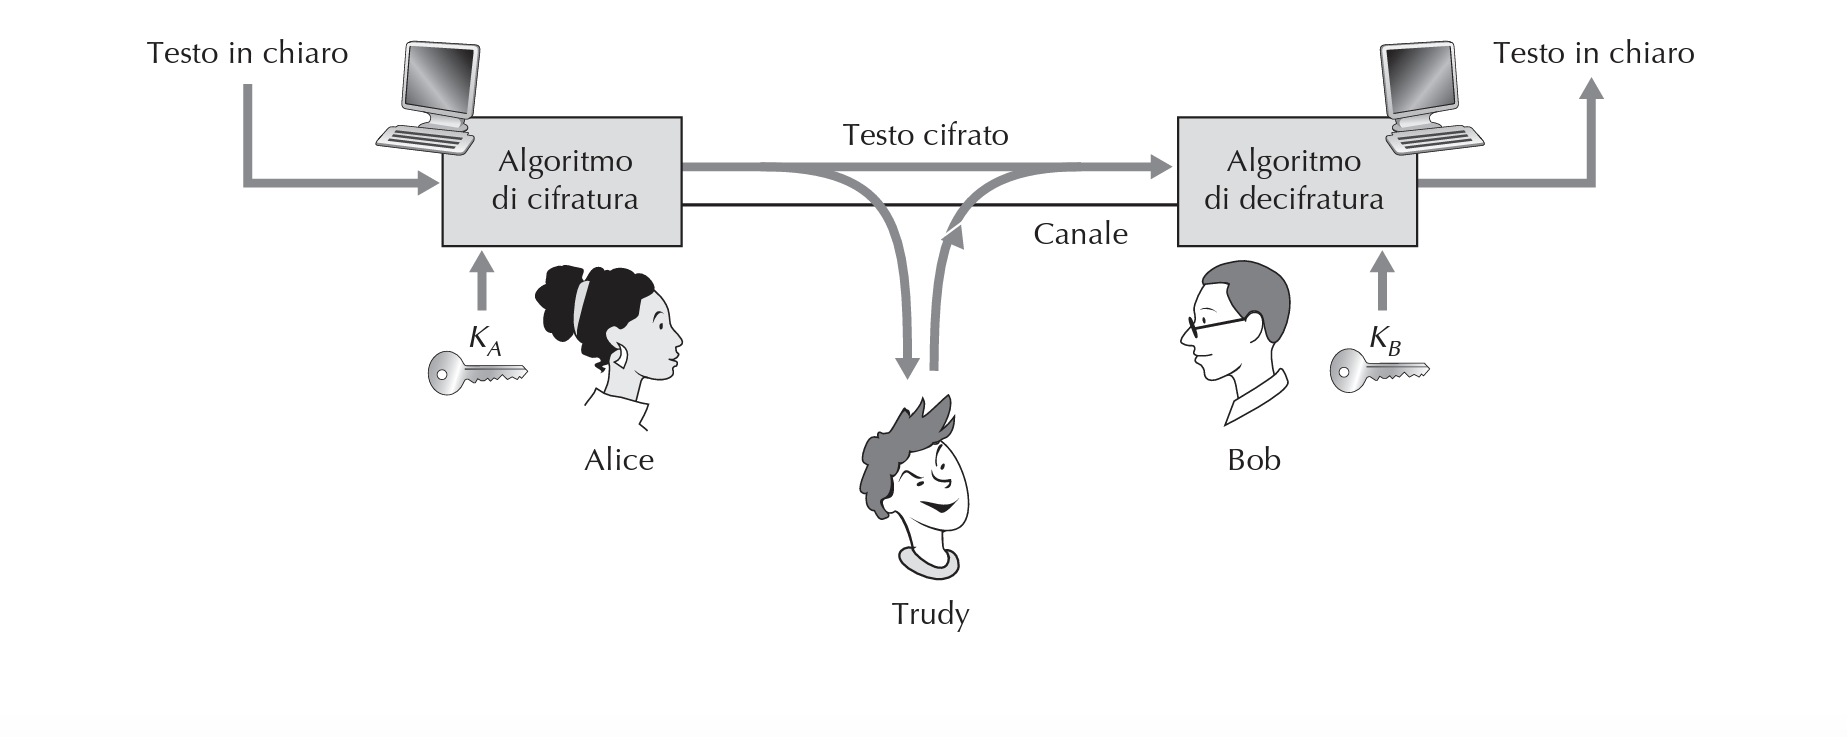
\includegraphics[width=12cm]{src/cifratura.png}
\end{figure}
\subsection{Elementi del processo crittografico}
Se le chiavi di cifratura e decifratura sono uguali: ha algoritmo simmetrico e la chiave 
deve essere segreta.
Se le chiavi sono diverse: l'algoritmo è asimmetrico e una chiave è pubblica, l'altra privata 
(\textit{e quindi segreta}).
\subsubsection{Robustezza crittografica}
Un algoritmo di cifratura è robusto se non è facilmente possibile:
\begin{itemize}
  \item Dato un testo cifrato ottenere il corrispondente testo in chiaro senza conoscere la chiave di decifratura.
  \item Dato un testo cifrato e il corrispondente testo in chiaro ottenere la chiave di decifratura.
\end{itemize}
In generale, nessun algoritmo crittografico è assolutamente sicuro, quindi si dice che è computazionalmente sicuro se:
\begin{itemize}
  \item Il costo necessario a violarlo è superiore al valore dell’informazione cifrata.
  \item Il tempo necessario a violarlo è superiore al tempo di vita utile dell’informazione cifrata.
\end{itemize}
\section{Crittoanalisi}
La crittoanalisi tenta di ricostruire il testo in chiaro senza conoscere la chiave di decifratura.
L'attacco più banale è quelli \textbf{a forza bruta}:
\begin{itemize}
  \item Tentare di decifrare il messaggio provando tutte le chiavi possibili. 
  \item Applicabile a qualunque algoritmo, ma la sua praticabilità dipende dal numero di chiavi possibili.
  \item È  comunque necessario avere informazioni sul formato del testo in chiaro, per riconoscerlo quando si trova la chiave giusta.
\end{itemize}
Principio di \textbf{Kerckhoffs}:
\begin{itemize}
  \item Nel valutare la sicurezza di un algoritmo crittografico si assume che il crittoanalista conosca tutti i dettagli dell’algoritmo.
  \item La segretezza deve risiedere nella chiave, non nell’algoritmo! 
\end{itemize}
\section{Crittografia a chiave simmetrica}
La crittografia simmetrica, altrimenti detta crittografia a chiave segreta,
utilizza una chiave comune e il medesimo algoritmo crittografico per
la codifica e la decodifica dei messaggi !

Due utenti che desiderano comunicare devono accordarsi su di un algoritmo e su di una chiave comuni,
La chiave deve essere scambiata su un canale sicuro.
\subsubsection{Cifratura di cesare}
Ogni carattere viene sostituito da un altro (\textit{permutazione}), secondo un certo alfabeto
che costituisce la chiave.
\[
\begin{matrix}
  \text{In chiaro}: && A B C D E F G H I L M N O P Q R S T U V Z \\
  \text{Cifrate}: &&  D E F G H I L M N O P Q R S T U V Z A B C  
\end{matrix}
\]
Le chiavi possibili sono solamente $20$.
\subsubsection{Cifratura monoalfabetica}
Ogni carattere viene sostituito da un altro (permutazione), secondo un certo alfabeto che costituisce la chiave 
\[
\begin{matrix}
  \text{In chiaro}: && A B C D E F G H I L M N O P Q R S T U V Z \\
  \text{Cifrate}: &&  M Z N C B V L A H S G D F Q P E O R I T U
\end{matrix}
\]
Le chiavi possibili sono pari al numero di permutazioni possibili $21!$,
ovvero $5.1 \cdot 10^{19}$.

\subsubsection{Anlisi delle frequenze}
Spazio delle chiavi di un algoritmo monoalfabetico molto grande, ma 
la crittoanalisi è semplice tramite l'analisi delle frequenze.

In un testo scritto in una determinata lingua (italiano, inglese...)
ogni lettera dell’alfabeto si presenta secondo una certa frequenza:

Ad esempio in italiano E ed A sono molto comuni, Q e Z sono poco comuni.
E poi ci sono gruppi di 2 o 3 lettere (“ch”, “che”, “qu”, \dots).

Contando il numero di occorrenze di ogni lettera nel testo cifrato è possibile ipotizzare
con buona probabilità quale sia la lettera corrispondente.
\subsubsection{Cifrari a blocchi}
Fa parte delle tecniche di cifratura simmetrica:
\begin{itemize}
  \item Usati in molti protocolli sicuri di Internet, compreso PGP (posta elettronica),
  SSL (connessione TCP) e IPSec (trasmissione a livello di rete).
  \item Chiamati anche cifrari a flusso.
\end{itemize}
Dati $k$ bit, i possibili $2^k$ ingressi vengono permutati, esempio $k=3$.
















\chapter{Wireshark}
TODO
\chapter{Docker}
\section{Motivazioni}
Gli hosts sono sempre connessi attraverso la rete che semplifica la distribuzione 
del software. Com'è possibile adattare tutti questi sistemi eterogenei con architetture, 
librerie e CPU diverse?

Le applicazioni di rete non sono ospitate in computer isolati, ma in:
\begin{itemize}
  \item Clusters: gruppi di decine di computers connessi con una LAN ad alte prestazioni.
  \item Data centers: gruppi di centinaia di computers connessi tramite una gerarchia 
  attraverso LAN ad alte prestazioni.
\end{itemize}
\section{Soluzioni}
Le soluzioni a questi problemi può passare attraverso:
\begin{itemize}
  \item La virtualizzazione: è il sistema più pulito per rendere il sistema il più 
  isolato possibile.
  \item Containers: cerca di semplificare la gestione attraverso l'eliminazione del sistema operativo 
  ospite e mantenendo solamente un sistema operativo per ogni applicazione e inserendo il container tra 
  il sistema operativo e le librerie utente.
\end{itemize}
Il container crea una membrana attorno ai processi per isolarli. Il programma è quindi 
scalabile, in questo modo posso gestire le risorse, è portabile (\textit{per ogni hardware viene 
distribuito l'immagine}).
\subsection{Ciclo di vita }
\begin{figure}[H]
  \centering
  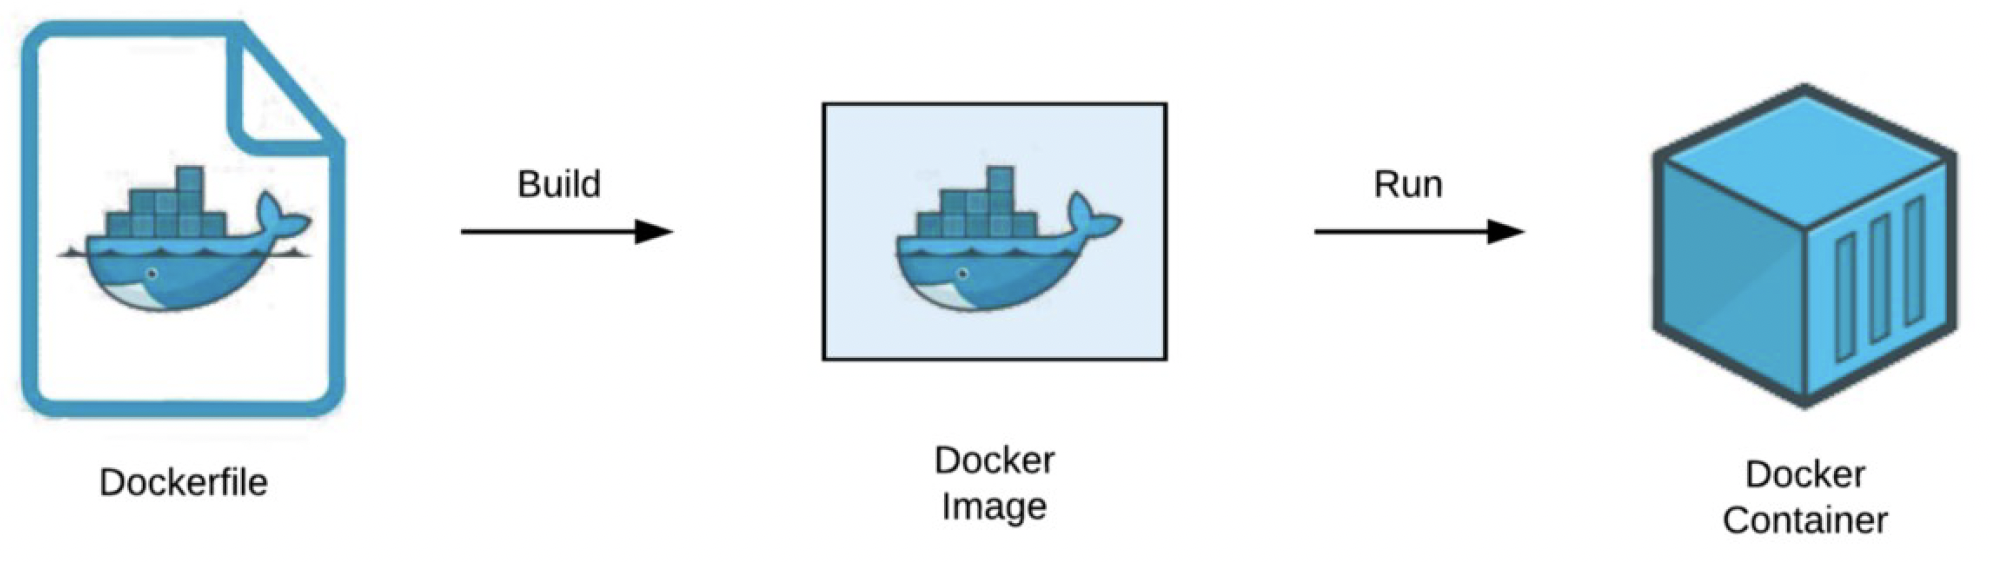
\includegraphics[width=10cm]{src/docker_img.png}
\end{figure}
\end{document}